\documentclass{article}
\usepackage{pgfplots}
\pgfplotsset{compat=1.17}

\begin{document}

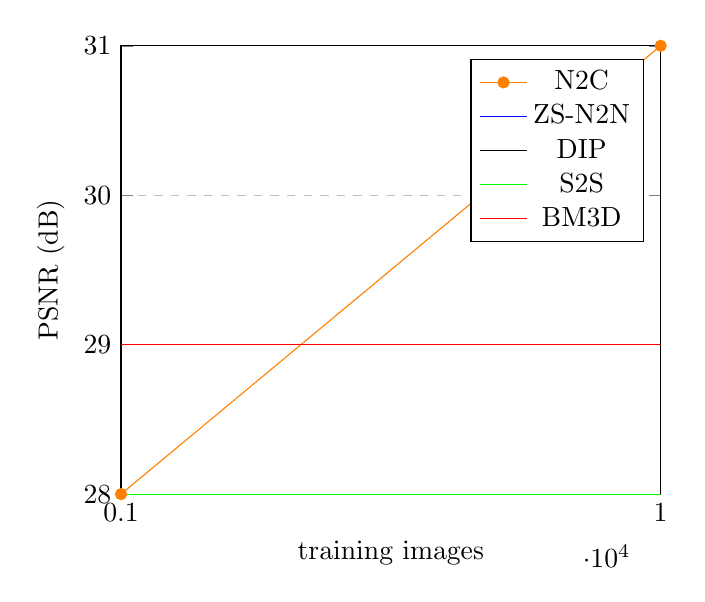
\begin{tikzpicture}
    \begin{axis}[
        xlabel={training images},
        ylabel={PSNR (dB)},
        xmin=1000, xmax=10000,
        ymin=28, ymax=31,
        xtick={1000, 10000},
        ytick={28, 29, 30, 31},
        legend pos=north east,
        ymajorgrids=true,
        grid style=dashed,
    ]
    
    % N2C
    \addplot[
        color=orange,
        mark=*,
        ]
        coordinates {
            (1000, 28)
            (10000, 31)
        };
        \addlegendentry{N2C}
        
    % ZS-N2N
    \addplot[
        color=blue,
        ]
        coordinates {
            (1000, 29)
            (10000, 29)
        };
        \addlegendentry{ZS-N2N}
        
    % DIP
    \addplot[
        color=black,
        ]
        coordinates {
            (1000, 29)
            (10000, 29)
        };
        \addlegendentry{DIP}
        
    % S2S
    \addplot[
        color=green,
        ]
        coordinates {
            (1000, 28)
            (10000, 28)
        };
        \addlegendentry{S2S}
        
    % BM3D
    \addplot[
        color=red,
        ]
        coordinates {
            (1000, 29)
            (10000, 29)
        };
        \addlegendentry{BM3D}
        
    \end{axis}
\end{tikzpicture}

\end{document}